\section{HDFS}

The Hadoop Distributed File System supports very large datasets. It differs from a relational database in that the data it stores is only semi-structured. The data is stored across multiple servers. In fact a single file can be split across multiple servers. This is made possible by Hadoop utilizes a master-slave configuration. The master is usually called "Name Node", the slaves are typically called "Data Nodes"

\subsection{Name Node}

The Name Node maintains a registry of the data in the distributed file system. Data in the HDFS is split up into blocks. The default size of each block is 128MB. For each block the Name Node will store an address of which Data Node the block is located on. When a request comes to the HDFS for a file, the Name Node will forward the request to each Data Node to gather each block and assemble the file. Due to the parallel nature of retrieval, throughput can be very high.

In figure \ref{fig:name-node} below we can see the Name Node on the left and our Data Nodes on the right. File 1 is split across nodes 1 and 4 and File 2 is split across nodes 3 and 4

\begin{figure}[H]
  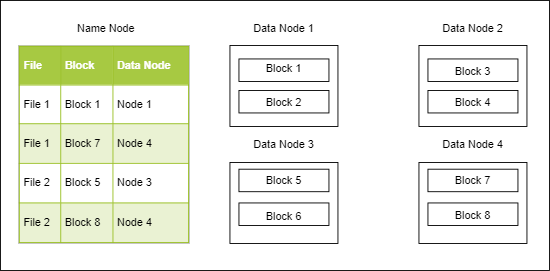
\includegraphics[width=\linewidth]{./images/name-node-data-node.png}
  \caption{Name Node and Data Nodes distribution}
  \label{fig:name-node}
\end{figure}

\subsection{Name Node Replication}

There is one drawback to only having one Name Node. If for some reason our Name Node goes down, all the data on the cluster is rendered useless. It would be impossible to reconstruct the data without the registry of each block of data. 

Luckily Hadoop has been built from the ground up with fault tolerance in mind. One of the reasons for this is that it has been designed to work on commodity hardware where faults are seen as a normal occurrence.

Hadoop has a number of mechanisms for ensuring data is fault tolerant. Including the following

\begin{itemize}
\item Fsimage and edits files
\item Secondary Name Node
\end{itemize}

FsImage is a complete snapshot of the HDFS at any point in time. This can also be referred to as a checkpoint. The edits file maintains a record of all changes to the HDFS since the last checkpoint. At regular intervals the edits file is combined with the previous checkpoint to create a new checkpoint. Using these 2 files it is possible to recover from failure and re-index the Name Node server. The default backup location for the FsImage file is on the name node server, however this location is configurable, so it could be on a remote hard drive. Reconstructing the data can take some time however and is very resource intensive because of the size of files we are dealing with.

A Secondary Name node is a simpler alternative. The is basically an exact copy of the primary name node. It maintains a backup of the FsImage and edits files and is synced in regular intervals with the primary Name Node. This again is called check-pointing. The frequency of check-pointing is also configurable. If an error occurs on the primary Name Node, our secondary Name Node is then promoted to be the primary Name Node.

